% ==================================================================================================================================
% Introduction à l'étude Qualitative

En pratique, on ne peut que très rarement résoudre formellement une équation différentielle. 
On va donc cherche, à partir de la fonction qui la définit, de déduire des propriétés sur les solutions. 

% ==================================================================================================================================
% Introduction à l'étude Qualitative

\section{Équations Autonomes}

\begin{definition}[Équation Autonome]
    Une équation différentielle est dite autonomme si elle est de la forme : 
        \[ (A) : y'(t) = f(y(t)) \] 
    Autrement dit si la variable temporelle (i.e $t$) n'apparaît pas dans $f$. 
\end{definition}

On peut interpréter une équation autonome en physique comme une équation à la contrainte de temps n'apparaît pas. 

Posons maintenant quelques définitions supplémentaires... 

\begin{definition}[Champ de vecteurs]
    Un champ de vecteurs est une fonction continue $f : \Omega \subset \R^n \longrightarrow \R^n$ où $\Omega$ est un ouvert. 
    Intuitivement, elle associe à chaque point de l'espace $\Omega$ un vecteur. 
\end{definition}

\begin{definition}[Courbe Intégrale]
    Une courbe intégrale d'un champ de vecteur $f : \Omega \longrightarrow \R^n$ est une \textbf{courbe paramétrée} 
    $y : I \subset \R \longrightarrow \Omega$ telle que $y$ est solution maximale de l'équation autonome :
        \[ (E) : y'(t) = f(y(t)) \quad \forall i \in I \] 
\end{definition}

\begin{definition}[Trajectoire]
    Une trajectoire de $f : \Omega \longrightarrow \R^n$ est l'image d'une courbe intégrale de $f$. 
\end{definition}

\begin{definition}[Point Stationnaire]
    On dit que $ x_0 \in \Omega$ est un point stationnaire ou point d'quilibre si $f(x_0) = 0$. 
    Un point stationnaire est un point où le champ de vecteur est nul. 
\end{definition}

Ainsi, un champ de vecteur va permettre de modéliser un système en mouvement tel que l'écoulement d'un fluide. 
Une trajectoire de ce champ de vecteur sera donc la trajectoire d'une particule dans le fluide. 

\begin{proposition}
    Soit $y$ une courbe intégrale d'une équation autonome $(A)$ alors si $c \in \R$ alors la courbe :
        \[ y_c : 
            \begin{cases}
                I + c \longrightarrow \R^n \\ 
                t \longmapsto y(t - c)
            \end{cases} \] 
    est une courbe intégrale (i.e solution maximale de $A$). Elle a la même trajectoire que $y$ à translation près. 
\end{proposition}

\begin{proposition}
    Soit $(A)$ une équation autonome définie par une fonction $f$. Supposons que $f$ est localement lispchitzienne. 
    Soient :
        \begin{align*}
            y_1 : I_1 \longrightarrow \R^n \\ 
            y_2 : I_2 \longrightarrow \R^n 
        \end{align*}
    deux solutions maximales de $(A)$ telles que 
        \[ \exists t_1, t_2 \in I_1, I_2, \quad y_1(t_1) = y_2(t_2) \] 
    \underline{alors} $y_1$ et $y_2$ sont égales à translation près. 
\end{proposition}

\begin{definition}[Orbite]
    Toutes les courbes intégrales $y$ d'une équation autonome $f$ vérifiant le même problème de Cauchy ont la même trajectoire. 
    Cette trajectoire est appelée \textbf{orbite}. 
    On appelle \textbf{portrait de phase} la partition de $\Omega$ en orbites.  
\end{definition}

\begin{prop}[Orbites]
    Deux orbites sont soient disjointes soient égales. 
\end{prop}

\begin{proposition}
    Soit $y$ une courbe intégrale d'une équation autonome $(A)$. On a : 
    \begin{itemize}
        \item Si $y$ admet une limite $l$ à l'infini, alors $l$ est un point stationnaire de. 
        \item Si $y$ n'est pas injective alors $y$ est globale et périodique. 
    \end{itemize}
\end{proposition}


% ==================================================================================================================================
% Intégrales Premières et Systèmes Hamiltoniens

\section{Intégrales Premières et Systèmes Hamiltoniens}

\subsection{Intégrales Premières et Courbes de Niveau}

\begin{definition}[Intégrale Première]
    Soit $(E) : y' = f(y)$ une équation autonome où $f : \Omega \overset{\text{L.L}}{\longrightarrow} \R^n$. 
    Une fonction $E : \Omega \overset{ \mathcal{C}^1}{\longrightarrow} \R$ telle que pour toute 
    solution $y$ de $(A)$, on ait $E \circ y = c \in \R $ 
    \begin{align*}
        \text{i.e } & \text{ pour toute courbe intégrale } (y,I), \forall t \in I, \quad \frac{\partial}{\partial t} E \circ y = 0 \\ 
        \text{i.e } & \quad \langle \nabla E, f \rangle = 0 \\ 
        \text{i.e } & E \text{ est constante le long des orbites}
    \end{align*}
    est appelée \textbf{intégrale première} de $(A)$. 
\end{definition}

En physique, les intégrales premières représentent les quantités invariances de systèmes dynnamiques représentés par des équations 
autonomes. Par exemple, dans un système fermé, un intégrale première peut représenter l'énergie du système.

\newpage 

\begin{proposition}[Lien équation autonome/système dynnamique]
    Dans la suite du chapitre, nous prendrons l'habitude d'écrire les équation autonomes sous forme de systèmes 
    dynnamiques (système d'équation différentielles). 
    Détaillons comment passer de l'un à l'autre dans la cas quelconque. 
    
    Soit $(A) : y' = f(y)$ une équation autonome où $f : \Omega \subseteq \R^n \longrightarrow \R^n$ et 
    $y = (y_1, \dots, y_n)$. Le système dynnamique associé est simplement l'équation différentielle noté : 
        \[ \frac{\partial}{\partial t} 
        \begin{pmatrix}
            y_1(t) \\ 
            \vdots \\ 
            y_n(t)
        \end{pmatrix}
        = 
        \begin{pmatrix}
            f_1(y_1(t), \dots, y_n(t)) \\ 
            \vdots \\ 
            f_n(y_1(t), \dots, y_n(t)) 
        \end{pmatrix} \] 
    Que l'on écrit plus généralement avec une lettre différente pour chaque composante de $y$. 
\end{proposition}

\begin{definition}[Courbe de Niveau]
    Soit $(A) : y' = f(y)$ une équation autonome où $f : \Omega \longrightarrow \R^n$. 
    Soit $E : \R^n \longrightarrow \R$ une intégrale première de $(A)$. 
    Les courbes de niveaux de $E$ sont les ensembles de points $y \in \R^n $ tels que 
        \[ E(y) = c \in \R \] 
\end{definition}

\begin{example}[Oscillateur Harmonique]
    Soit l'équation différentielle autonome suivante : 
        \[ (A) : 
            \begin{cases}
                x'(t) = v(t) \\
                v'(t) = - \omega ^2 x(t)
            \end{cases}
            \quad \forall (t,\omega) \in \R \times \R \] 
    ici, $x$ représente la position d'un oscillateur et $v$ sa vitesse. 
    Une intégrale première de ce système est de la forme : 
        \[ E : 
            \begin{cases}
                R \times \R \overset{ \mathcal{C}^1}{\longrightarrow} \R \\ 
                (x,y) \longmapsto E(x,y) 
            \end{cases} \] 
    Multiplions $(A)$ par $v$. On a alors $ \forall t \in \R$ : 
        \begin{align*}
            v(t) v'(t) &= - \omega ^2 x(t)v(t) \\ 
            &= - \omega ^2 x(t)x'(t) \\ 
            \iff & v(t) v'(t) + \omega ^2 x(t) x'(t) = 0 
        \end{align*}
    Supposons que $E$ soit de la forme : $ \forall t \in \R, E : (x(t), v(t)) \longmapsto E(x(t), v(t))$.
    D'après la règle de la chaîne, on a $ \forall t \in \R$ : 
        \begin{align*}
            \frac{\partial}{\partial t} E(x(t), v(t)) &= \frac{\partial x(t)}{\partial t} \frac{\partial E}{\partial x} + \frac{\partial v(t)}{\partial t} \frac{\partial E}{\partial y}
            = x'(t) \frac{\partial E}{\partial x} + v'(t) \frac{\partial E}{\partial y}  \\
            \Longrightarrow & \frac{\partial E}{\partial x} = \omega ^2 x(t) \quad \text{et} \quad \frac{\partial E}{\partial y} = v(t) 
        \end{align*}
        On peut donc en conclure que : 
            \[ \forall t \in \R, \quad E(x(t), v(t)) = \frac{1}{2} \omega^2 x^2(t) + \frac{1}{2} v^2(t) \]  
    Réciproquement, par construction, $ \frac{\partial E}{\partial t} = 0 $. 
    Traçons maintenant quelques courbes de niveau : 
    
    \begin{center}
        \begin{minipage}{0.35\textwidth}
            \centering
            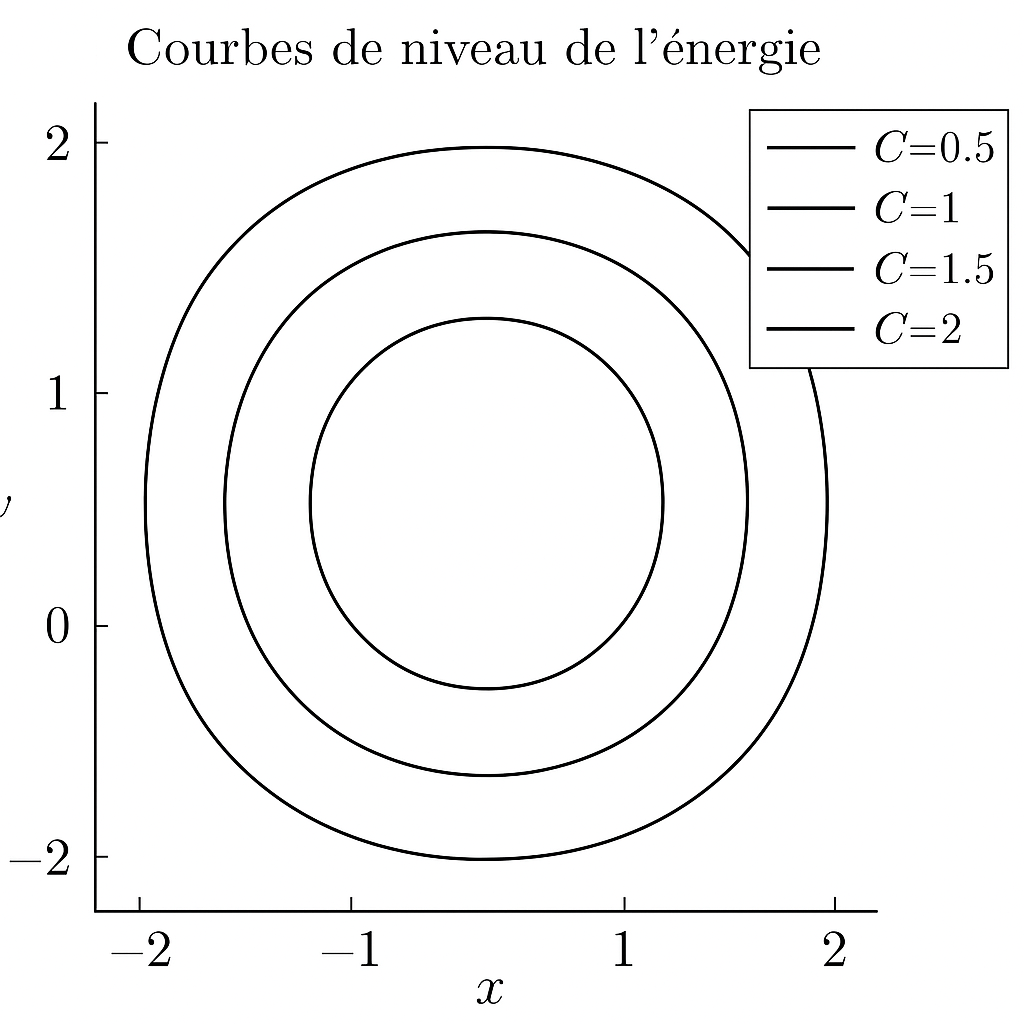
\includegraphics[scale=0.1]{./images/courbes_niveaux.png}
        \end{minipage}
        \hfill 
        \begin{minipage}{0.55\textwidth}
            Ces courbes permettent de représenter l'évolution du mouvement de l'oscillateur dans le plan. 
            Ici, plus l'énergie $C$ est élevée, plus le rayon des cercles en grand, 
            ce qui correspond à une plus grande amplitude. 

            On peut aussi les voir comme l'ensemble des orbites pour lesquelles l'énergie est égale à $C$. 
        \end{minipage}
    \end{center}
\end{example}

\begin{prop}[Orbites et Ensemble de Niveau]
    Toute orbite est incluse dans un ensemble de niveau. 
\end{prop}

Ainsi, les intégrales premières d'équations autonomes $(A)$ permettent de donner une idée de la forme des orbites formés
par les solutions de $(A)$. 

\subsection{Systèmes Hamiltoniens}

Il existe un cas particulier des équations autonomes appelés systèmes hamiltoniens. Ils offrent une approche plus 
simple pour l'étude des systèmes dynnamiques conservatifs, où certaines quantités sont conservées au cours du temps. 

\begin{definition}[Système Hamiltonien]
    Un système hamiltonien est une équation différentielle autonome (ou système d'équations différentielles autonomes associé) 
    pouvant être représentée par un fonction appelée \textbf{hamiltonien}. 
    Plus formellement, soit $(A) : y' = f(y)$ une équation autonome telle que $f : \Omega \longrightarrow \R^{2n}$. 
    On dit que $(A)$ est un système hamiltonien s'il existe une fonction : 
    \[ H : 
        \begin{cases}
            \Omega \overset{ \mathcal{C}^2}{\longrightarrow} \R \\ 
            (q,p) \longmapsto H(q,p) 
        \end{cases} 
        \quad \text{où } q,p \in \R^n \] 
    telle que $ \forall (q,p) \in \Omega$ on ait : 
        \[ \boxed{f(q,p) = \left( \frac{\partial H}{\partial p}, - \frac{\partial H}{\partial q} \right)  } \] 
    Cela revient donc à dire que $(A)$ peut s'écrire de la forme suivante : 
        \[ (A) : 
            \begin{cases}
                p'(t) = - \partial_q H(q,p) \\ 
                q'(t) = \partial_p H(q,p) 
            \end{cases} \] 
\end{definition}

\begin{remark}
    Tout système de dimension impaire n'est donc pas hamiltonien. 
\end{remark}

\begin{example}[Oscillateur Harmonique]
    Prenons comme exemple le cas classique d'un oscillateur harmonique gouverné par l'équation 
    différentielle : 
        \[ (A) : m x'' + kx = 0 \] 
    où : 
    \begin{itemize}
        \item $m$ est la masse de l'oscillateur 
        \item $k$ est la constante de raideur du ressort 
        \item $x(t)$ est la position de l'oscillateur à l'instant $t$. 
    \end{itemize}
    Représentons cette équation autonome sous la forme d'un système hamiltonien. 
    Posons $Y(t) = (x(t), y(t))$ on a alors $Y'(t) = (x'(t), y'(t))$. Soit la fonction suivante : 
    \[ f : 
        \begin{cases}
            \R^2 \longrightarrow \R^2 \\ 
            (x,y) \longmapsto (y, - \frac{k}{m}x)
        \end{cases} \] 
    Cela nous donne que : 
        \begin{align*}
            (A) \iff & Y'(t) = f(Y(t)) \\ 
            \iff & 
                \begin{cases}
                    x'(t) = y(t) \\ 
                    y'(t) = - \frac{k}{m} x 
                \end{cases} 
            \iff  
                \begin{cases}
                    x'(t) = \frac{1}{m} p(t) \\ 
                    p'(t) = -kx(t) 
                \end{cases}
        \end{align*}
        où $ p(t) = m x'(t)$ 
    
    Maintenant, posons : 
        \[ H : 
            \begin{cases}
                \R^2 \longrightarrow \R \\ 
                (x,p) \longmapsto \frac{p^2}{2m} + \frac{1}{2} k x^2 
            \end{cases} \] 
    $H$ est $ \mathcal{C}^\infty$ par composantes donc calculons ses dérivées partielles : 
        \[ \frac{\partial H}{\partial p} = \frac{p}{m} = x'(t) \quad \frac{\partial H}{\partial x} = k x(t) = - p'(t) \] 
    Donc $(A)$ est bien un système hamiltonien. 
\end{example}

\begin{prop}[Hamiltonien et intégrale première]
    Tout hamiltonien est une intégrale première. Autrement dit, un hamiltonien est un cas particulier d'intégrale première. 
\end{prop}

\begin{proposition}[Condition Nécessaire]
    Soit $(A) = y' = f(y)$ un système hamiltonien, alors $ \div f = 0 $. 
    En dimension 2, on a équivalence. 
\end{proposition}




